%!TEX root = main_arduino_intro.tex

\chapter{Display}

In order to display the temperature of our sample cooling setup, we will connect a display to our Arduino. Displays come in many shapes and forms, form the monitor you might be reading this on to simple \ac{led} seven-segment displays. An overview of various displays that are ready to be deployed on Arduino can, e.g., be found \href{https://www.arduino.cc/reference//en/libraries/category/display/}{here}. For our specific case, a simple seven-segment display will do the trick to display the temperature.

\subsection{Seven-segment displays} 

\begin{figure}[htb]
    \centering
    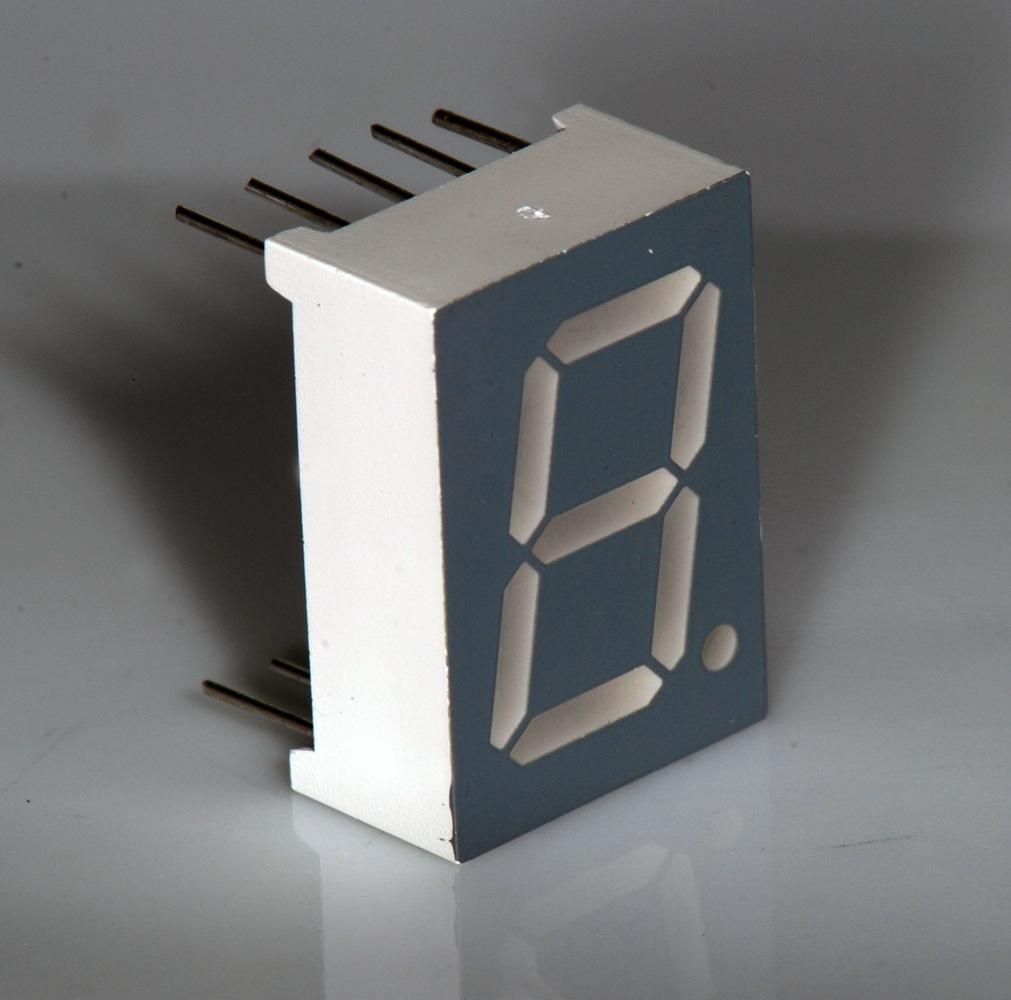
\includegraphics[height=4cm]{graphics/02_display/7seg_photo.jpg} \hspace{1.5cm}
    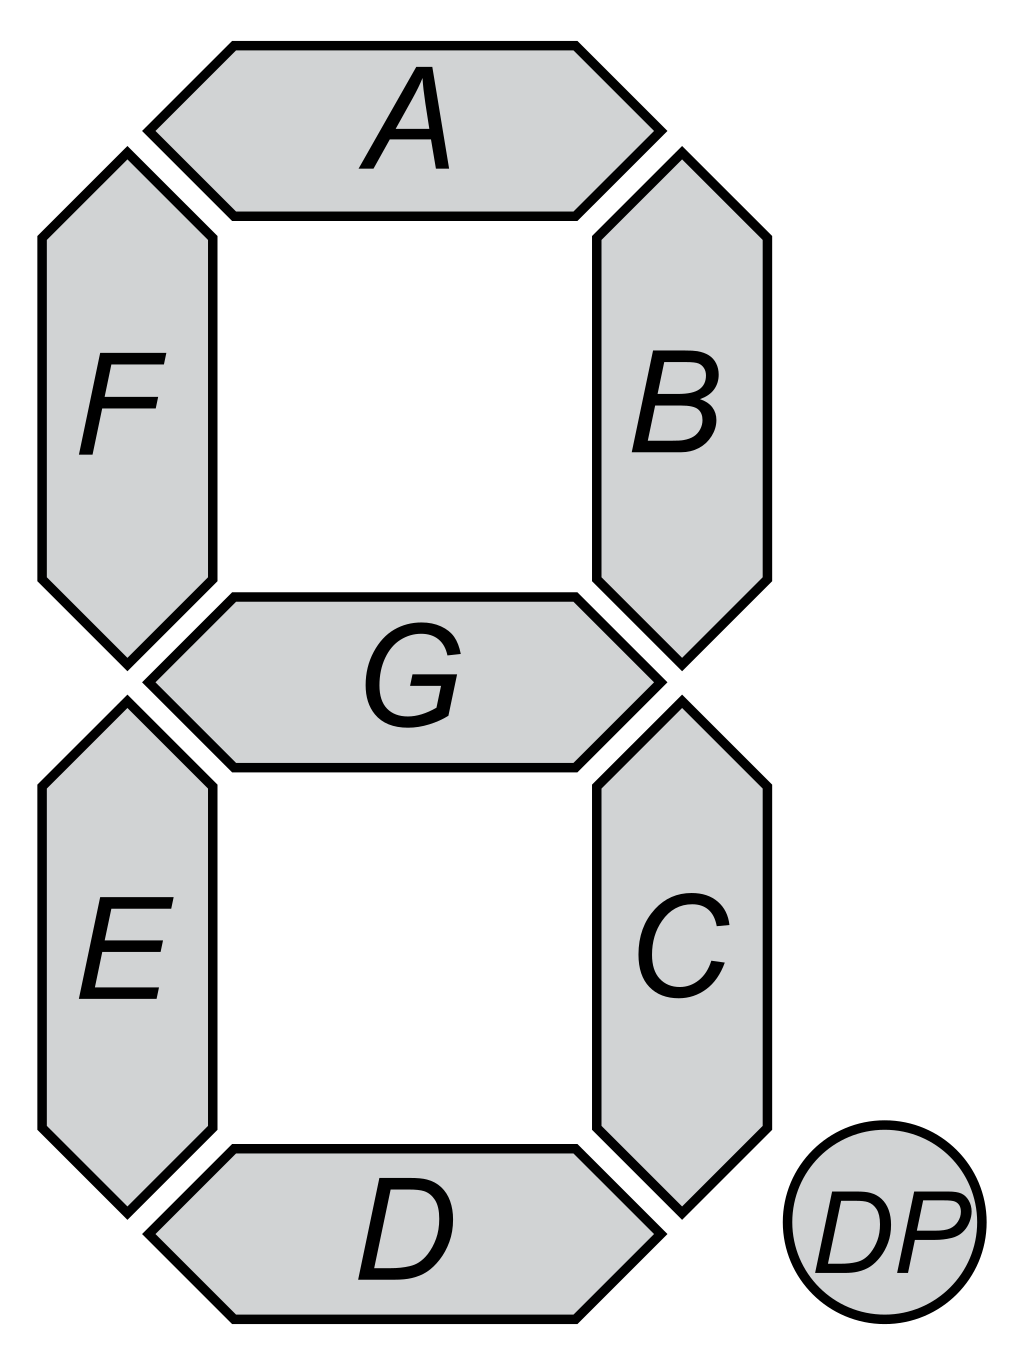
\includegraphics[height=4cm]{graphics/02_display/7seg_schematic.png}
    \caption{Seven-segment display: photo (left) and schematic (right). Credit: \href{https://en.wikipedia.org/wiki/Seven-segment_display\#/media/File:Seven_segment_01_Pengo.jpg}{Peter Halasz (left)} and \href{https://en.wikipedia.org/wiki/Seven-segment_display\#/media/File:7_Segment_Display_with_Labeled_Segments.svg}{Uln2003 (right)} via Wikipedia. License: \href{https://creativecommons.org/licenses/by-sa/3.0/}{CC by SA-3.0 (left)}, \href{https://en.wikipedia.org/wiki/Seven-segment_display\#/media/File:7_Segment_Display_with_Labeled_Segments.svg}{Public domain -- CC0 (right)}}
    \label{fig:display:7seg}
\end{figure}
As displayed in Figure~\ref{fig:display:7seg}, seven-segment displays contain seven individual segments that allow us to display any number and even some letters. In addition, they usually contain a decimal point. The right-hand figure shows the schematic and typical labeling of a seven-segment display. Each segment is its own \ac{led} and we could drive these \acp{led} by using multiple \ac{io} pins. However, in order display multiple numbers, the number of \ac{io} pins that we would use up would very fast become too extensive. Figure~\ref{fig:display:7seg} shows that the seven-segment display has five pins on top and, not shown here, also five connectors on the bottom. For each seven-segment display you could look up the wiring diagram and notice that each segment has its own connection and that they have a total of two common grounds.

Chips such as a 74HC595 that allow us to convert serial into parallel data allow us to effectively control multiple outputs, as required for such a display, while only using a a few pins.
\begin{figure}[tb]
    \centering
    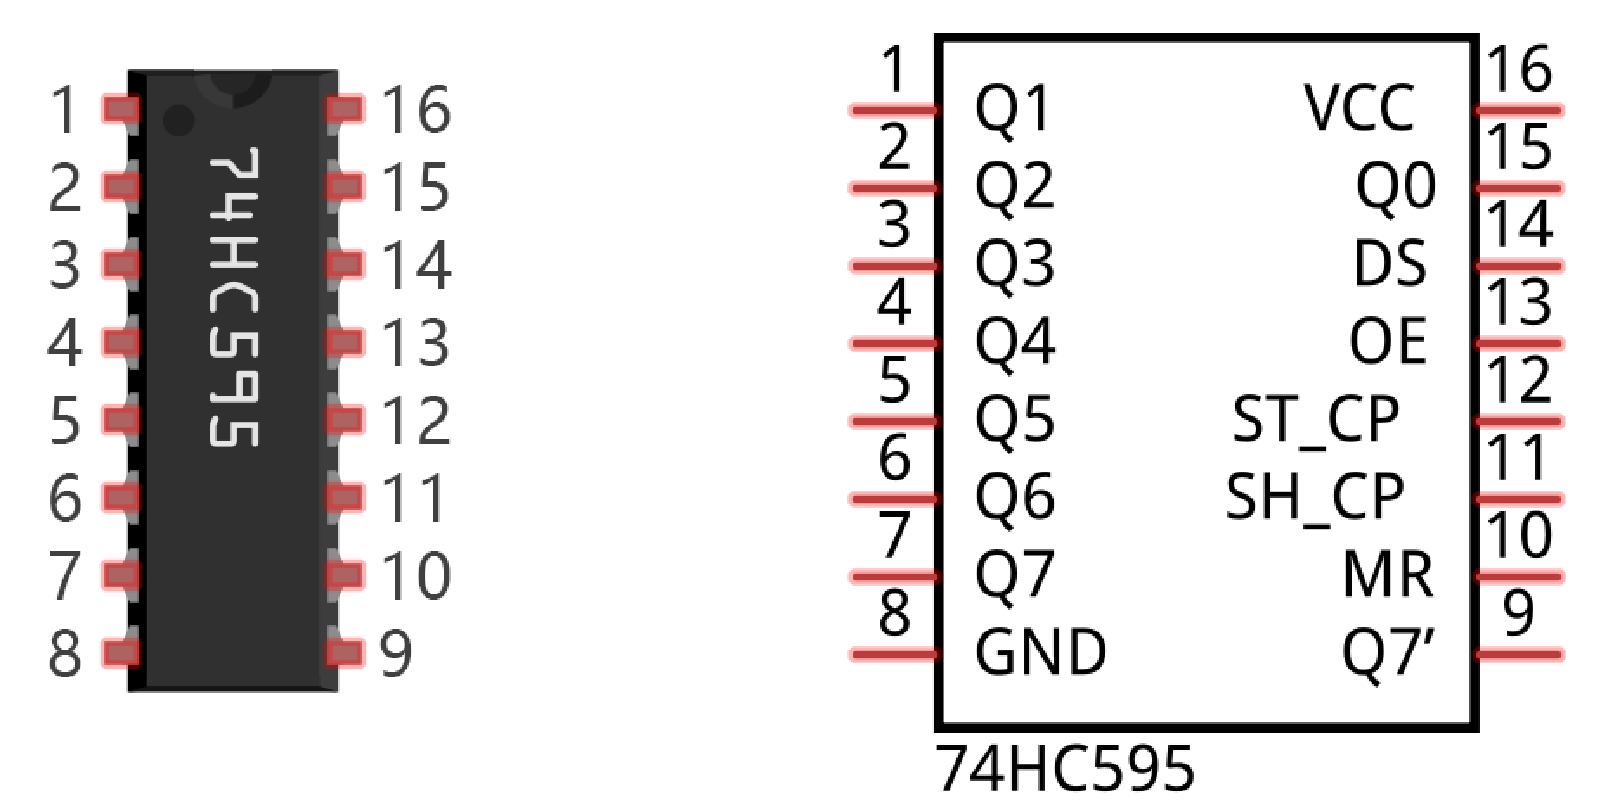
\includegraphics[]{graphics/02_display/74hc595.png}
    \caption{Schematic and pin names of a 74HC595 chip. Credit: \href{https://github.com/Freenove/Freenove_Ultimate_Starter_Kit}{Freenove}, License: \href{https://www.creativecommons.org/licenses/by-nc-sa/3.0/deed.en_US}{CC BY-NC-SA 3.0}}
    \label{fig:display:74hc595}
\end{figure}
Figure~\ref{fig:display:74hc595} shows a schematic and pin names of such a chip. Note the notch on the top of the schematic that each chip contains in order to provide you with a reference on the pin assignments. You can in fact find various versions of this chip from different manufacturers, e.g., the data sheet for the Texas Instruments version can be found \href{https://www.ti.com/lit/ds/symlink/sn74hc595.pdf?ts=1636228778140&ref_url=https%253A%252F%252Fwww.google.com%252F}{here}. Generally, the pins have the following purposes:

\begin{center}
\begin{tabular}{lll}
    \hline
    \textbf{Pin name}   &   \textbf{Pin number} &   \textbf{Description}    \\
    \hline \hline
    Q0 - Q7             &   1-7, 15             &   Parallel data output \\
    GND                 &   8                   &   Ground \\
    Q7'                 &   9                   &   Serial data output \\
    MR                  &   10                  &   Remove shift register \\
    SH\_CP              &   11                  &   Serial shift clock \\
    ST\_CP              &   12                  &   Parallel update output \\
    OE                  &   13                  &   Enable output \\
    DS                  &   14                  &   Serial data input \\
    \hline
\end{tabular}
\end{center}

As indicated by the names, the parallel data output pins are the eight pins that can be connected to the individual \acp{led} of a seven-segment system. The GND pin provides the ground connection of the chip. The serial data output (Q7') can be used to connect another 74HC595 chip in series. The MR and SH\_CP take care of clearing the shift register and timing when a shift happens. The ST\_CT triggers an update in the parallel output and the OE pin enables this output. Finally, the DS pin is where the serial input is given. 

\morebox{Want do build your own seven segment display driver?}{Detailed instructions on how to use a 74HC595 chip to drive a seven segment display can be found online, e.g., on in chapter 15 of \href{https://github.com/Freenove/Freenove_Ultimate_Starter_Kit/blob/master/Tutorial.pdf}{this tutorial}. Building such a driver is outside the scope of our workshop, however, it might be useful for you to read and understand the shifting itself and how it works. Please have a look at the mentioned tutorial.}


\section{Adafruit four-digit, seven-segment display with backpack}

As described above, we could build our own driver for a seven-segment display. However, it seems to be fairly cumbersome to develop such a driver, especially since low-cost, pre-fabricated displays with communication ``backpacks'' exist. Here, we will use an \href{https://www.adafruit.com/product/1002}{Adafruit four-digit, seven-segment display} that communicates with the Arduino via the \ac{i2c} communications protocol.

\infobox{\ac{i2c} protocol}{\Ac{i2c} is a single ended, synchronous, multi-controller/multi-target, single bus communication protocol and is ideally suited for integrated microelectronics. The following figure shows the configuration with one microcontroller and three selected devices. (Credit: \href{https://en.wikipedia.org/wiki/I\%C2\%B2C\#/media/File:I2C_controller-target.svg}{Tim Mathias}, License: \href{https://creativecommons.org/licenses/by-sa/4.0/}{CC BY-SA 4.0})
\vspace{-0.5cm}
\begin{center}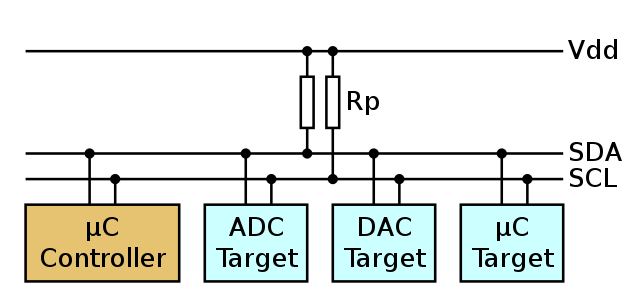
\includegraphics[width=0.5\textwidth]{graphics/02_display/i2c.png}\end{center}
The microcontroller connects to each device via a data (SDA) and a clock line (SCL). Furthermore, power (Vdd) and ground (GND) are connected as well; to light our \acp{led} we need power. The clock defines the timing of commands, i.e., triggers sending / receiving and the data line sends the required commands. More details on the \ac{i2c} communication protocol can be found on \href{https://en.wikipedia.org/wiki/I\%C2\%B2C}{Wikipedia}.}


\subsection{Assembly}

\begin{figure}[htb]
    \centering
    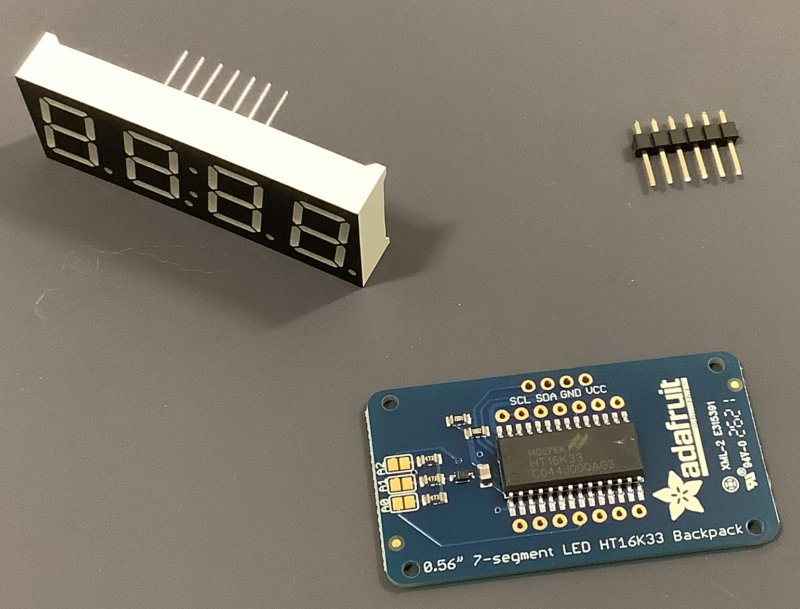
\includegraphics[width=0.4\textwidth]{graphics/02_display/7seg_adafruit_unpacked.jpg}
    \caption{Parts of the four-digit, seven-segment display.}
    \label{fig:display:7seg_unpacked}
\end{figure}
The four-digit, seven-segment display package requires assembly by soldering. Figure~\ref{fig:display:7seg_unpacked} shows the individual components of the display that need to be soldered together. On the top left is the display itself. The backpack is shown on the bottom and the header pins, which allow us to connect the display to the breadboard, are shown on the top right. If you have never soldered before, please review the \href{https://www.youtube.com/watch?v=AqvHogekDI4}{this video} that will show you some best practices. Generally, remember to:
\begin{itemize}
    \item Avoid excessive amounts of solder
    \item Ensure good contact between your component and the \ac{pcb}
    \item Double check your parts orientation
\end{itemize}

\infobox{Types of soldering}{The two types of soldering generally referred to are through hole and surface mount soldering. In this workshop we will only perform through-hole soldering, i.e., we will stick the leads / pins through the \ac{pcb} and solder from the other side in order to ensure a connection. Surface mount soldering mounts components on top of \acp{pcb}. A great tutorial video for this type can be found \href{https://www.youtube.com/watch?v=f9fbqks3BS8}{here}.}

One of the great features when using components and kits from Adafruit is that they have very detailed instructions. All instructions for the four-digit, seven-segment display can be found \href{https://learn.adafruit.com/adafruit-led-backpack/0-dot-56-seven-segment-backpack}{here}.

\exerbox{Assemble the display kit by following the \href{https://learn.adafruit.com/adafruit-led-backpack/0-dot-56-seven-segment-backpack-assembly}{Adafruit assembly instructions}. Double, then triple check the orientation of the display prior to soldering; it is difficult to remove the display after soldering and resolder it in the correct orientation. (In fact, I experienced this last part the hard way. Right after I wrote\break
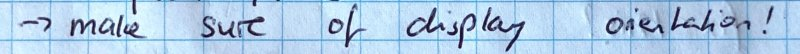
\includegraphics[width=0.75\textwidth]{graphics/02_display/orientation_reminder.jpg}\break
I soldered the display onto the \ac{pcb} the wrong way around\dots)}


\subsection{Controlling the display from Arduino}

As for the assembly, Adafruit has detailed instructions on how to connect and control the display. In fact, they even provide an Arduino library that allows us to easily control the display (this was one of the reasons for choosing this display to start with). \href{https://learn.adafruit.com/adafruit-led-backpack/0-dot-56-seven-segment-backpack-arduino-setup}{This tutorial} goes in detail through the setup for Arduino, including a how-to for installing the libraries. For reference, Figure~\ref{fig:display:7seg_connected} shows an image of the display connected to the Arduino. 

\begin{figure}[htb]
    \centering
    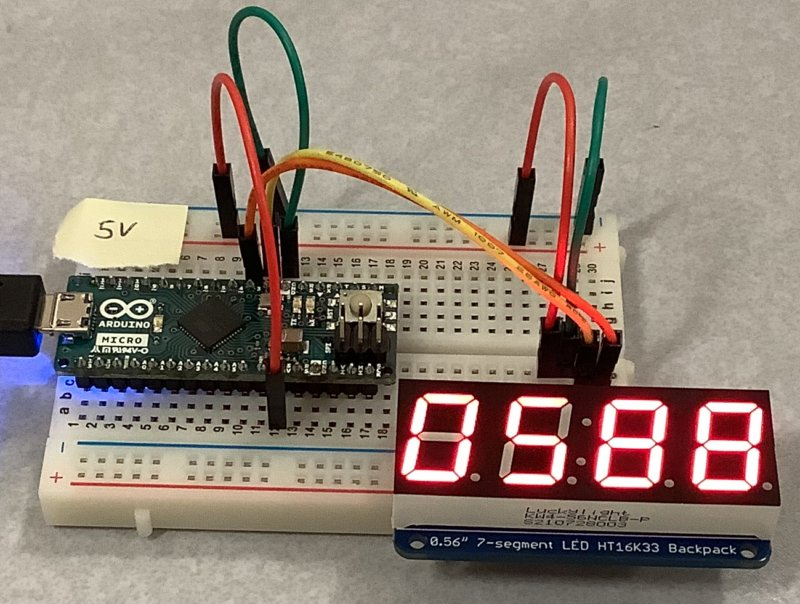
\includegraphics[width=0.5\textwidth]{graphics/02_display/7seg_adafruit_connected.jpg}
    \caption{The display connected to the Arduino Micro on a breadboard.}
    \label{fig:display:7seg_connected}
\end{figure}

\exerbox{Go through the \href{https://learn.adafruit.com/adafruit-led-backpack/0-dot-56-seven-segment-backpack-arduino-setup}{Adafruit tutorial} to connect the display to your Arduino. Then ensure that it works as expected by running the example script that Adafruit provides. Various different ways are given in the tutorial. Make sure you understand the different ways of controlling the display. Feel free to modify the example and display your own values.}

\exerbox{For our final setup we want the display to display the current temperature (2 digits plus +/- sign) and the set point if this is changed by pressing a button. Write a subroutine that takes two input arguments and allows you display the following values: \lstinline{"  -9"}, \lstinline{"  20"}, \lstinline{"s-10"}. The last example is for displaying the setpoint with an additional \lstinline{s} in front of it (which is equal to \lstinline{5}). \textit{Hint}: Your subroutine might start with something like this: \break\lstinline{void dispTemp(int temperature, bool setPoint) \{...\}}}
